\documentclass{scrartcl}
\usepackage{amsmath}
\usepackage{amssymb}
\usepackage[geometry]{ifsym}
\usepackage{tikz}
\usetikzlibrary{positioning,calc}
\usepackage{xfrac}

\newcommand{\selection}{\sigma}
\newcommand{\projection}{\pi}
\newcommand{\rename}{\rho}
\newcommand{\join}{\mathbin{\text{\begin{tiny}\textifsym{|><|}\end{tiny}}}}
\newcommand{\fullouterjoin}{\mathbin{\text{\begin{tiny}\textifsym{d|><|d}\end{tiny}}}}
\newcommand{\semijoin}{\mathbin{\text{\begin{tiny}\textifsym{|><}\end{tiny}}}}
\newcommand{\groupby}{\Gamma}

\newcommand{\mtt}[1]{\text{\texttt{#1}}}

\setlength{\parindent}{0pt}

\begin{document}

\section*{Exercise 1}

Label nodes breadth-first:

\begin{table}[h]
\begin{tabular}{l|l}
Relation & Label \\ \hline
$R_0$ & 0 \\
$R_1$ & 2 \\
$R_2$ & 3 \\
$R_3$ & 1 \\
$R_4$ & 4
\end{tabular}
\end{table}

This results in the following graph:

\begin{tikzpicture}
    \node (L0) {0};
    \node (L2) [right=of L0] {2};
    \node (L4) [right=of L2] {4};
    \node (L1) [below=of L0] {1};
    \node (L3) [right=of L1] {3};
    \draw
        (L0) edge (L2)
        (L2) edge (L4)
        (L0) edge (L1)
        (L2) edge (L3)
        (L1) edge (L3);
\end{tikzpicture}

The DPccp algorithm gives us the following ccp of labels:

\begin{table}[h]
\begin{tabular}{ll}
Connected subraphs & Complementary subgraphs \\ \hline\hline
$\{4\}$ & \\ \hline
$\{3\}$ & \\ \hline
$\{2\}$ & $\{4\}$ \\
& $\{3\}$ \\ \hline
$\{2, 3\}$ & $\{4\}$ \\ \hline
$\{2, 4\}$ & $\{3\}$ \\ \hline
$\{2, 3, 4\}$ & \\ \hline
$\{1\}$ & $\{3\}$ \\
& $\{2,3\}$ \\
& $\{2,3,4\}$ \\ \hline
$\{1, 3\}$ & $\{2\}$ \\
& $\{2,4\}$ \\ \hline
$\{1, 2, 3\}$ & $\{4\}$ \\ \hline
$\{1, 2, 3, 4\}$ \\ \hline
$\{0\}$ & $\{2\}$ \\
& $\{2, 3\}$ \\
& $\{2, 4\}$ \\
& $\{2, 3, 4\}$ \\
& $\{1\}$ \\
& $\{1, 3\}$ \\
& $\{1, 2, 3\}$ \\
& $\{1, 2, 3, 4\}$
\end{tabular}
\end{table}
\begin{table}[h]
\begin{tabular}{ll}
Connected subraphs & Complementary subgraphs \\ \hline\hline
$\{0, 1\}$ & $\{3\}$ \\
& $\{2\}$ \\
& $\{2, 3\}$ \\
& $\{2, 4\}$ \\
& $\{2, 3, 4\}$ \\ \hline
$\{0, 2\}$ & $\{4\}$ \\
& $\{3\}$ \\
& $\{1\}$ \\
& $\{1, 3\}$ \\ \hline
$\{0, 1, 2\}$ & $\{4\}$ \\
& $\{3\}$ \\ \hline
$\{0, 1, 3\}$ & $\{2\}$ \\
& $\{2, 4\}$ \\ \hline
$\{0, 2, 3\}$ & $\{4\}$ \\
& $\{1\}$ \\ \hline
$\{0, 2, 4\}$ & $\{3\}$ \\
& $\{1\}$ \\
& $\{1, 3\}$ \\ \hline
$\{0, 2, 3, 4\}$ & $\{1\}$ \\ \hline
$\{0, 1, 2, 3\}$ & $\{4\}$ \\ \hline
$\{0, 1, 2, 4\}$ & $\{3\}$ \\ \hline
$\{0, 1, 2, 3, 4\}$
\end{tabular}
\end{table}

\section*{Exercise 2}

At the beginning we have the following ordering benefits:

\begin{table}[h]
\begin{tabular}{lll}
$\join_1$ & $\join_2$ & orderingBenefit($\join_1$, $\join_2$) \\ \hline
$R_0 \join R_3$ & $R_0 \join R_1$ & $\sfrac{150}{101}$ \\
$R_1 \join R_2$ & $R_1 \join R_0$ & $\sfrac{5}{3}$ \\
$R_1 \join R_4$ & $R_1 \join R_0$ & $\sfrac{500}{251}$ \\
$R_1 \join R_4$ & $R_1 \join R_2$ & $\sfrac{300}{251}$ \\
$R_2 \join R_3$ & $R_2 \join R_1$ & $\sfrac{5}{4}$ \\
$R_3 \join R_0$ & $R_3 \join R_2$ & $2$
\end{tabular}
\end{table}

So we chose to run $R_3 \join R_2$ before $R_3 \join R_0$. This results in the
following graph:

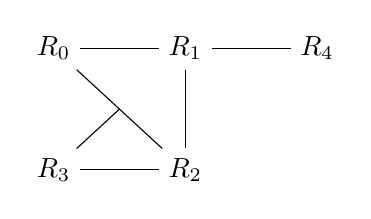
\begin{tikzpicture}
    \node (R0) {$R_0$};
    \node (R1) [right=of R0] {$R_1$};
    \node (R4) [right=of R1] {$R_4$};
    \node (R3) [below=of R0] {$R_3$};
    \node (R2) [right=of R3] {$R_2$};
    \draw
        (R0) edge (R1)
        (R1) edge (R4)
        ($(R0)!0.5!(R2)$) edge (R0) edge (R2) edge (R3)
        (R1) edge (R2)
        (R3) edge (R2);
\end{tikzpicture}

\pagebreak

Update the table:

\begin{table}[h]
\begin{tabular}{lll}
$\join_1$ & $\join_2$ & orderingBenefit($\join_1$, $\join_2$) \\ \hline
$R_0 \join \{R_2, R_3\}$ & $R_0 \join R_1$ & $\sfrac{85}{37}$ \\
$R_1 \join R_2$ & $R_1 \join R_0$ & $\sfrac{5}{3}$ \\
$R_1 \join R_4$ & $R_1 \join R_0$ & $\sfrac{500}{251}$ \\
$R_1 \join R_4$ & $R_1 \join R_2$ & $\sfrac{300}{251}$ \\
$R_2 \join R_3$ & $R_2 \join R_1$ & $\sfrac{5}{4}$
\end{tabular}
\end{table}

Next we chose to order $R_0 \join R_1$ before $R_0 \join \{R_2, R_3\}$. This
results in the following graph:

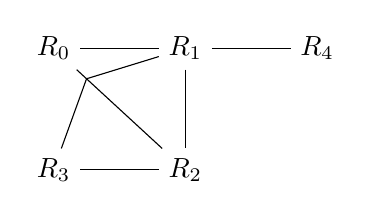
\begin{tikzpicture}
    \node (R0) {$R_0$};
    \node (R1) [right=of R0] {$R_1$};
    \node (R4) [right=of R1] {$R_4$};
    \node (R3) [below=of R0] {$R_3$};
    \node (R2) [right=of R3] {$R_2$};
    \draw
        (R0) edge (R1)
        (R1) edge (R4)
        ($(R0)!0.25!(R2)$) edge (R0) edge (R2) edge (R3) edge (R1)
        (R1) edge (R2)
        (R3) edge (R2);
\end{tikzpicture}

\end{document}
